\documentclass[border=4pt]{standalone}
\usepackage[T1]{fontenc}
\usepackage{helvet}
\renewcommand{\familydefault}{\sfdefault}
\usepackage{graphicx}
\usepackage{caption}
\usepackage{amsmath}
\captionsetup{font={sf,footnotesize},labelfont={sf,bf,footnotesize},justification=justified,singlelinecheck=false}
\begin{document}
\setcounter{figure}{0}
\begin{minipage}{7.20in}
\centering
\begin{figure}[htbp]
    \centering
    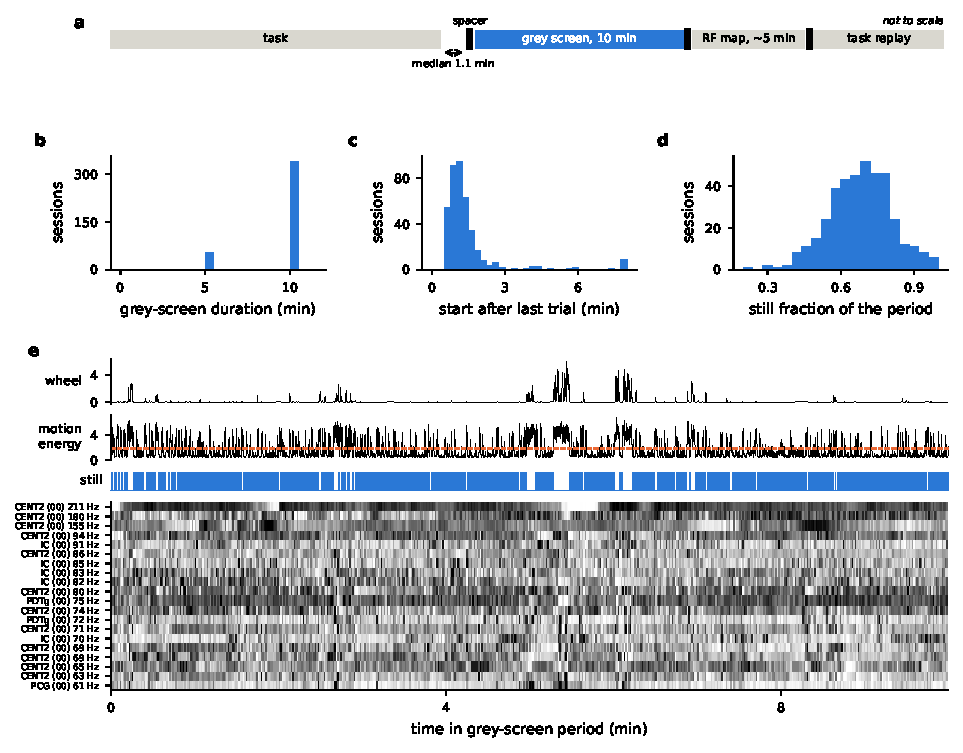
\includegraphics[width=\linewidth]{fig1_protocol_panels.pdf}
    \caption{\textbf{a} IBL passive protocol after the task (iblrig \texttt{passiveChoiceWorld}): frame2ttl spacers separate the spontaneous period, during which Bonsai clears the screen to grey with the sync square off and shows no stimulus (\texttt{SPONTANEOUS\_ACTIVITY\_SECONDS} = 600), receptive-field mapping (sparse noise) and the replay of task stimuli, valve clicks and tones. Task length is schematic. The interval comes from \texttt{\_ibl\_passivePeriods.intervalsTable}. \textbf{b} Grey-screen duration over the 396 BWM sessions (130 mice) that have it; 600 s in 86\%. \textbf{c} Delay between the end of the last task trial and the start of the grey screen (values above 8 min clipped). \textbf{d} Fraction of the period that is still: 50 ms bins without wheel movement ($>$0.05 rad/s), licks or motion energy above the session's 60th percentile, with a one-bin margin (the first second is skipped); median 6.5 min of 10. In the 35 sessions without motion energy, stillness rests on wheel and licks only (median fraction 0.81 vs 0.67). \textbf{e} Example session with median stillness: wheel speed, left-camera motion energy (normalised to the session median; dashed, the stillness threshold; wheel in rad/s), the resulting still bins, and a raster of the 20 neurons with the highest firing rate in this window (of 236 good units on both probes; 0.5 s bins, each row scaled between its 1st and 99th percentile, black = high; labels give Beryl region, probe and mean rate). This session's probes are in cerebellum and brainstem, so these are not DMN neurons.}
    \label{fig:grey_protocol}
\end{figure}
\end{minipage}
\end{document}
